\section{Collisioni in ALICE}
In questa sezione si cerca di introdurre la fisica delle collisioni riguardanti le collisioni ultrarelativistiche di ioni.

Nel Modello Standard si descrivono tre delle quattro forze fondamentali: la forza forte, la forza elettromagnetica, la forza debole in ordine di intensità.
Dalla teoria della cromodinamica quantistica (QCD) si sa che ogni nucleone è composto da quark, i quali interagiscono tramite l'interazione forte attraverso lo scambio di gluoni.
Dalla QCD inoltre sappiamo che il gluone in realtà non è altro che un quanto di energia dei campi mediatori della forza forte, e tramite un'invarianza di gauge locale SU(3) si ricavano 8 tipi di gluoni, tutti con carica di colore diversa in modo da formare una base per coprire tutti i colori possibili.\\

\subsection{Il sistema pre-collisione}
Per ricreare le condizioni richieste per la formazione di QGP è possibile far collidere ioni pesanti a regime ultra-relativistico.
In questo regime, con la contrazione di Lorentz lungo la direzione del fascio, gli ioni appaiono come dei dischi piatti (\autoref{fig:pb}), e per questo motivo le dimensioni trasversali del nucleo appaiono più larghe delle dimensioni longitudinali. 
Perciò una collisione tra ioni può essere considerata come la sovrapposizione di collisioni individuali tra i nucleoni provenienti da direzioni opposte.
\begin{figure}[htb]
    \centering
    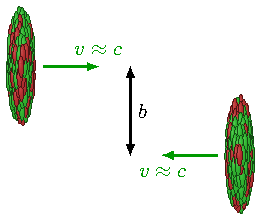
\includegraphics[width=0.5\textwidth]{image/1-alice/PbPb_collisions.pdf}
    \caption{Schema rappresentativo di una collisione Pb-Pb. Le sfere rosse rappresentano i protoni e le sfere verdi i neutroni. (Autore: \href{https://tikz.net/pbpb_collisions/}{Izaak Neutelings})}
    \label{fig:pb}
\end{figure}

È importante notare che non sempre tutti i nucleoni partecipano alla collisione: questo succede se nel piano del fascio i baricentri dei nuclei non non coincidono ma sono separati da una distanza $b$ (parametro di impatto), in questo caso interagiranno soltanto i nucleoni all'interno dell'area di sovrapposizione nucleare. 
I nucleoni non interagenti sono chiamati \emph{spettatori}; i nucleoni che viceversa partecipano alla collisione vengono chiamati \emph{partecipanti}.
Se il numero di nucleoni partecipanti è $N_\text{part}$, il numero di spettatori è $N_\text{spect} = 2A-N_\text{part}$.
Il parametro d'impatto $b$ gioca un ruolo fondamentale nelle collisioni di nuclei: esso determina la centralità di una collisione, una quantificazione della regione di sovrapposizione, e con ciò il numero di nucleoni partecipanti.
%Da questo si può capire che, se si vuole più statistica, è necessario minimizzare questo parametro massimizzando così la centralità della collisione.
Dal momento che la centralità è correlata con la molteplicità di una collisione, ossia il numero di particelle cariche prodotte nella collisione, affinché si possa normalizzare le osservabili tra collisioni differenti, la misura della centralità è fondamentale.

Vi sono due metodi principali per la misura della centralità:
\begin{itemize}
    \item Il primo metodo consiste nella misura diretta della molteplicità, tramite conteggio del numero di particelle cariche prodotte in una collisione.
    Questo metodo è tuttavia dipendente dalla scelta del modello geometrico utilizzato per i processi adronici;
    \item il secondo metodo invece si basa sulla misura dell'energia degli spettatori, in genere effettuata in posizioni di alta molteplicità.
    Questo modello, al contrario del primo, è indipendente dal modello di collisione utilizzato.
\end{itemize}

\subsection{Il sistema post-collisione}
Grazie all'alta densità di energia che si viene a creare nell'urto ultra-relativistico tra ioni pesanti, si viene a formare un sistema che interagisce per l'interazione forte, il QGP.
Lo studio di questo sistema è proprio l'obiettivo di ALICE, ossia quello di andare a indagare lo stato del QGP.
In questo stato l'energia del sistema rende l'interazione forte meno dominante, portando a uno stato deconfinato di materia in cui i quark e i gluoni possono muoversi liberamente.
\begin{figure}[htb]
    \centering
    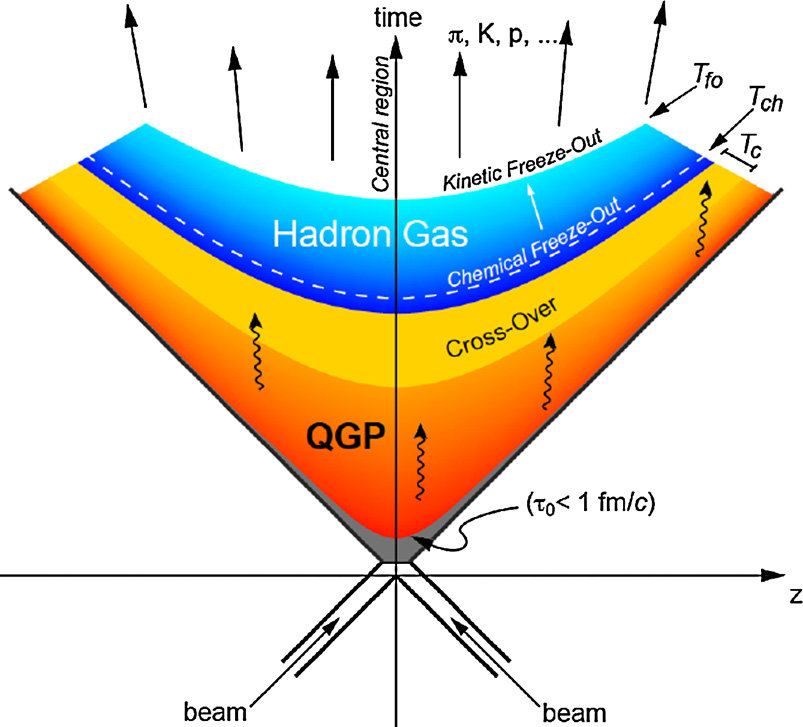
\includegraphics[width=0.7\textwidth]{image/1-alice/Colour-online-Space-time-diagram-of-a-heavy-ion-collision-of-two-nuclei-colliding-at.jpg}
    \captionwithsource{Diagramma spazio-tempo di una collisione di due ioni pesanti ultra-relativistici. La zona grigia sottostante alla QGP rappresenta lo stato di pre-equilibro.}{\cite{QGPbraun}}
    \label{fig:qgp}
\end{figure}

Più precisamente, al momento dell'impatto degli ioni, le singole collisioni coinvolgono scattering "hard" ovvero con un alto trasferimento di impulso che inducono alla produzione di partoni ad alta energia.
In questo momento si distinguono due zone in particolare: la prima a rapidità centrale, dove si è depositata la maggior parte dell'energia, la seconda invece ad alta rapidità, popolata da quark di valenza e particelle spettatori.
Nella zona a rapidità centrale, se la densità di energia è sufficientemente alta, si forma il QGP, sotto forma di \emph{fireball} in equilibrio termico.
In questa fase di equilibrio la \textit{fireball} si espande per via della pressione esercitata alla sua superficie e di conseguenza si ha un calo progressivo della temperatura; una volta che la temperatura sarà scesa al di sotto del valore critico inizia il processo di adronizzazione.
Successivamente, non appena lo scambio di impulso diventa insufficiente per sostenere le interazioni inelastiche, allora si arriva al cosiddetto \emph{freeze-out chimico}, in cui le abbondanze relative delle particelle rimangono invariate.
Nel momento in cui le particelle prodotte non interagiscono più, conservando il loro quadrimpulso, allora si parla di \emph{freeze-out cinetico}.
Infine, dopo $\sim15$ fm/$c = 5\cdot 10^{-23}$ s gli adroni formatisi giungono ai rilevatori.
Uno schema spazio-tempo di quanto appena descritto è rappresentato in \autoref{fig:qgp}.